% example tikz figure

\documentclass{article}

\usepackage{tikz}
\usetikzlibrary{arrows,shapes,positioning,shadows,trees}


\begin{document}

\begin{tikzpicture}
    % x-axis with length 6, label point O below (0,0), no arrow for x-axis
    \draw[-] (-3,0) -- (3,0);
    % \node[below] at (0,0) {$O$};
    % label O with a cross
    \node[fill,circle,inner sep=1pt,label=below:$O$] at (0,0) {};
    % label -R and R at point (-2,0) and (2,0) respectively
    \node[fill,circle,inner sep=1pt,label=below:$-R$] at (-2,0) {};
    \node[fill,circle,inner sep=1pt,label=below:$R$] at (2,0) {};

    % circle from R to -R, with label \gamma_R and arrow on it
    \draw[->] (2,0) arc (0:180:2);
    \node[label=above right:$\gamma_R$] at (2*0.6,2*0.8) {};
    % arrow
    \draw[->] (2*0.6 + 0.1 * 0.8, 2*0.8 - 0.1 * 0.6)-- (2*0.6,2*0.8);
\end{tikzpicture}

\begin{tikzpicture}
    % x-axis with length 6, label point O below (0,0), no arrow for x-axis
    \draw[-] (-3,0) -- (3,0);
    % \node[below] at (0,0) {$O$};
    % label O with a cross
    \node[fill,circle,inner sep=1pt,label=below:$O$] at (0,0) {};
    % label -R and R at point (-2,0) and (2,0) respectively
    \node[fill,circle,inner sep=1pt,label=below:$-R$] at (-2,0) {};
    \node[fill,circle,inner sep=1pt,label=below:$R$] at (2,0) {};

    % circle from R to -R, with label \gamma_R and arrow on it
    \draw[->] (2,0) arc (0:180:2);
    \node[label=above right:$\gamma_R$] at (2*0.6,2*0.8) {};
    % arrow
    \draw[->] (2*0.6 + 0.1 * 0.8, 2*0.8 - 0.1 * 0.6)-- (2*0.6,2*0.8);

    % label i at (0,1)
    \node[fill,circle,inner sep=1pt,label=right:$i$] at (0,1) {};
\end{tikzpicture}


\begin{tikzpicture}
    % x-axis with length 8
    \draw[-] (-4,0) -- (4,0);
    % origin, -R&R at (-3,0)&(3,0)
    \node[fill,circle,inner sep=1pt,label=below:$O$] at (0,0) {};
    \node[fill,circle,inner sep=1pt,label=below:$-R$] at (-3,0) {};
    \node[fill,circle,inner sep=1pt,label=below:$R$] at (3,0) {};

    % y-axis with length 3, only +y
    \draw[->] (0,0) -- (0,2.5);

    % label i\pi at (0,1)
    \node[fill,circle,inner sep=1pt,label=right:$i\pi$] at (0,1) {};

    % label 2i\pi at (0,2)
    \node[fill,circle,inner sep=1pt,label=above right:$2i\pi$] at (0,2) {};

    % \gamma_1 from R to (3,2)
    \draw[->] (3,0) -- (3,1);
    \draw[-] (3,1) -- (3,2);
    \node[label=above right:$\gamma_1$] at (3,1) {};

    % \gamma_2 from (3,2) to (-3,2)
    \draw[->] (3,2) -- (2,2);
    \draw[-] (2,2) -- (-3,2);
    \node[label=above right:$\gamma_2$] at (2,2) {};

    % \gamma_3 from (-3,2) to (-3,0)
    \draw[->] (-3,2) -- (-3,1);
    \draw[-] (-3,1) -- (-3,0);
    \node[label=above left:$\gamma_3$] at (-3,1) {};
\end{tikzpicture}

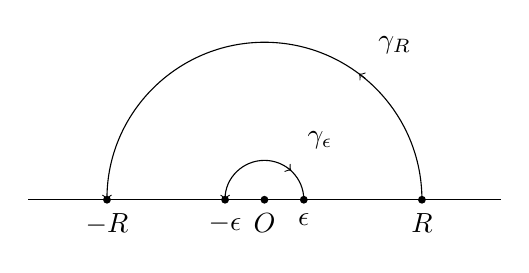
\begin{tikzpicture}
    % x-axis with length 6, label point O below (0,0), no arrow for x-axis
    \draw[-] (-3,0) -- (3,0);
    % \node[below] at (0,0) {$O$};
    % label O with a cross
    \node[fill,circle,inner sep=1pt,label=below:$O$] at (0,0) {};
    % label -R and R at point (-2,0) and (2,0) respectively
    \node[fill,circle,inner sep=1pt,label=below:$-R$] at (-2,0) {};
    \node[fill,circle,inner sep=1pt,label=below:$R$] at (2,0) {};

    % circle from R to -R, with label \gamma_R and arrow on it
    \draw[->] (2,0) arc (0:180:2);
    \node[label=above right:$\gamma_R$] at (2*0.6,2*0.8) {};
    % arrow
    \draw[->] (2*0.6 + 0.1 * 0.8, 2*0.8 - 0.1 * 0.6)-- (2*0.6,2*0.8);

    % likewise, draw from (-0.5,0) -> (0.5,0), each label -\epsilon and \epsilon
    \node[fill,circle,inner sep=1pt,label=below:$-\epsilon$] at (-0.5,0) {};
    \node[fill,circle,inner sep=1pt,label=below:$\epsilon$] at (0.5,0) {};
    \draw[->] (0.5,0) arc (0:180:0.5);
    \node[label=above right:$\gamma_\epsilon$] at (0.5*0.6,0.5*0.8) {};
    \draw[->] (0.5*0.6,0.5*0.8) -- (0.5*0.6 + 0.05*0.8, 0.5*0.8 - 0.05*0.6);
\end{tikzpicture}
\end{document}